\documentclass[]{report}   % list options between brackets
\usepackage{}              % list packages between braces
\usepackage{graphicx}
\usepackage[margin=1in]{geometry}
\usepackage{listings}

\lstset{frame = single}


%\usepackage[letterpaper, portrait, margin=1in]{geometry}



% type user-defined commands here

\begin{document}

\renewcommand{\chaptername}{Part}

%\title{Gonzaga Men's Basketball Yahtzee Game}   % type title between braces
%\author{Tom Scavo}         % type author(s) between braces
%\date{October 27, 1995}    % type date between braces
%\maketitle


\begin{titlepage}
    \centering
   
    \vfill
    
    
\includegraphics[width=6in]{Graphics/1718PosterPhoto.jpg} % also works with logo.pdf
    
    {\bfseries\Huge
        Gonzaga Men's Basketball\\
        Yahtzee Game\\
    }   
    
    {\bfseries\huge
        \vskip.5in
        Final Report \\
    }     
    
    {\bfseries\Large
       \vskip1in
        Gonzaga University\\
        CPSC 224-02\\
        Spring 2018\\
        Dr. Yanping Zhang\\
      
        \vskip.5in
        Benjamin Bladow\\
        Eugene Krug\\
        Brandon Niblock
    }    
   
    \vfill
    \vfill
    \vfill
\end{titlepage}


\chapter{Introduction}             % chapter 1
\section{Problem Statement}     % section 1.1

We were tasked with taking a traditional Yahtzee game, making modifications, and implementing it using a Graphical User Interface (GUI) in the Java programming language. One of the most significant modifications in our game is a theme. Our group elected to use the Gonzaga Men's Basketball team as our theme. We implemented the theme throughout the game. Some highly visible examples of the theme include the fifteen-sided die with each side of the die representing a player on the 2017-2018 team roster. The implementation of the theme will be made more clear throughout this report and in the game. This a multi-user game that tracks users' scores and maintains a leaderboard. For the purposes of clarity,  in this final report ``user" refers to the people playing the game and ``player" refers to a Gonzaga Men's Basketball Player. 


\section{Game Rules}       % section 1.2
\begin{itemize}

\item \textbf{The Dice}
\begin{itemize}
\item The game uses five, fifteen-sided dice.
\item The sides of each die represent the GU Men's Basketball 2017-2018 Roster: 
\begin{center}
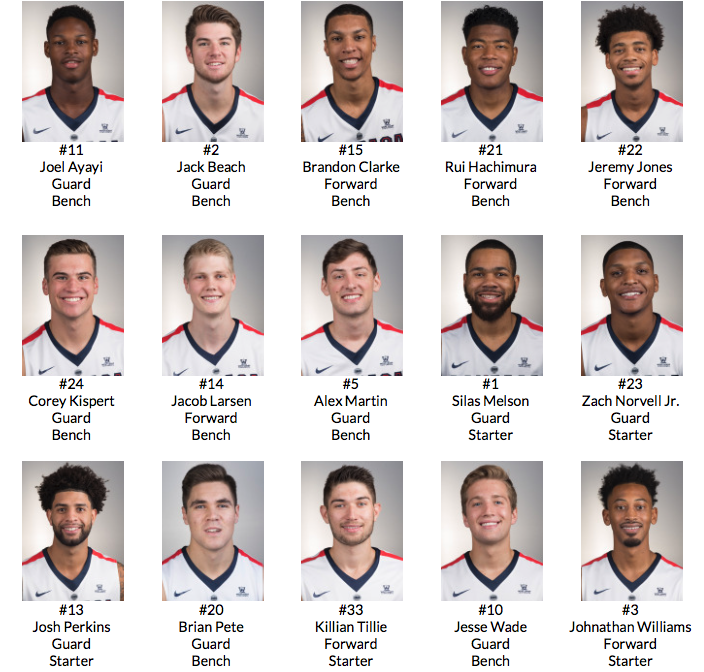
\includegraphics[width=3.7in]{Graphics/RosterScreenshot}
\end{center}
\end{itemize}

\item \textbf{How to Win}
\begin{itemize}
\item Roll dice 5 times to get the highest score after all 22 rounds.
\end{itemize}

\item \textbf{How to Play}
\begin{itemize}
\item To start, users will roll the dice by clicking the basketball image. After rolling users can either score the current roll on the scorecard by click ``Finishing Turn" or reroll any or all of the dice*. Users may only roll the dice a total of five times. After the fifth roll users must choose a line on the scorecard to score their hand in. Users must choose a different line each time (i.e. users CANNOT score their hand in a line they have already scored.)
\item To keep a player, users click their picture. Not clicking a picture will cause that die to be rerolled. For example, if the roll is Jones, Hachimura, Norvell, Tillie, Perkins to keep Jones, Norvell, and Tillie and reroll the others you would: click, not click, click, click, and not click.
\item *Note: For example, after the first roll users can keep 4 dice and reroll the fifth die. Then users can choose to keep all of the die and end that round or keep the first 2 die and roll the next 3 and continue...

\end{itemize}

\item \textbf{Scoring}
\begin{itemize}
\item \textbf{Upper Section}
\begin{itemize}
\item Each line in the upper section is calculated by the number of the player rolled multiplied by its scaling factor (1-15) as outlined on the scorecard. For example, two Brian Petes in a hand would be of value 24 (2 x 12 = 24).
\end{itemize}
\item \textbf{Lower Section}

\begin{itemize}
\item \textbf{3 of a Zag:} A user must have 3 of the same player in their hand. The score is the value of all 5-dice added up.
\item \textbf{4 of a Zag:} A user must have 4 of the same player in their hand. The score is the value of all 5-dice added up.
\item \textbf{Full Team:} A user must have 3 Guards and 2 Forwards to accomplish this score. The score will be 25 points, regardless of the players number values.
\item \textbf{The Bench Brigade:} A user must have 5 players from the Bench to accomplish this score. The score will be 30 points, regardless of players number values.
\item \textbf{The Starters:} A user must have all 5 Starters to accomplish this score. The score will be 40 points, regardless of players' number values.
\item \textbf{The Kennel:} No combos necessary. The score of this roll will be all the players' numbers totaled together.
\item \textbf{Zombie Nation:} A user must have 5 of the same player to accomplish this score. The score will be 100 points, regardless of players' number values.
\end{itemize}

\vspace{2.3in}
\item \textbf{Scorecard}
\begin{center}
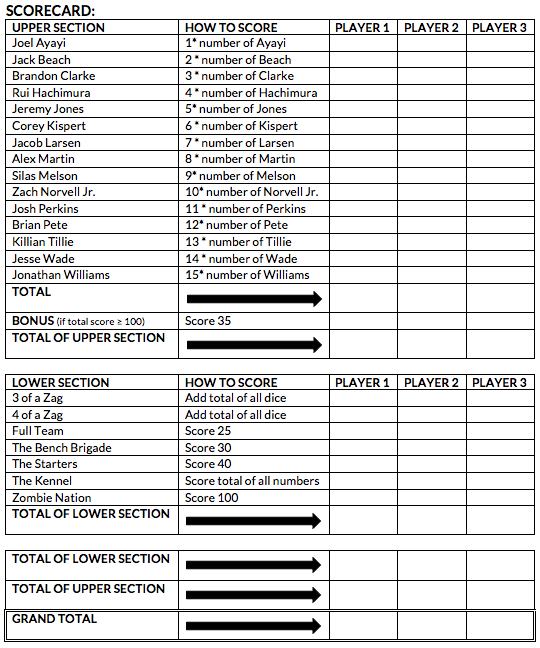
\includegraphics[width=5in]{Graphics/ScorecardScreenshot}
\end{center}
\end{itemize}
\end{itemize}


\chapter{Program Design and Implementation}           % chapter 2
\section{UML Class Diagram}     % section 2.1
There is one exception to our rule of the distinction between ``user" and ``player". We have a ``Player" class that should be named ``User" class instead. The exception is in our code and reflected in both of the diagrams. This exception to our rule exists because of legacy code from Programming Assignment 6.
\begin{center}
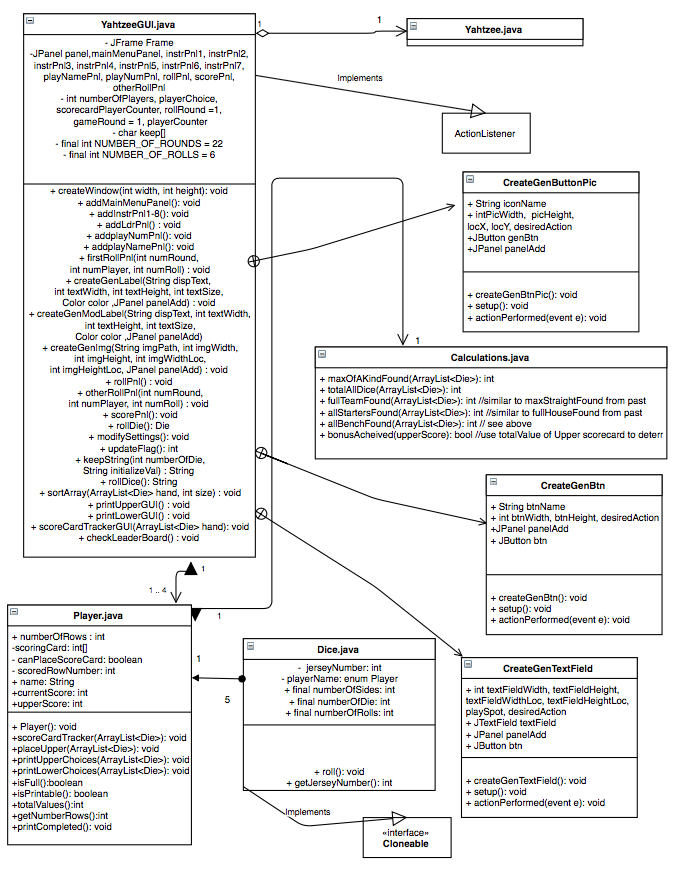
\includegraphics[width=4.3in]{Graphics/UMLClassDiagramScreenshot.png}
\end{center}
\section{UML Sequence Diagram}     % section 2.2
\begin{center}
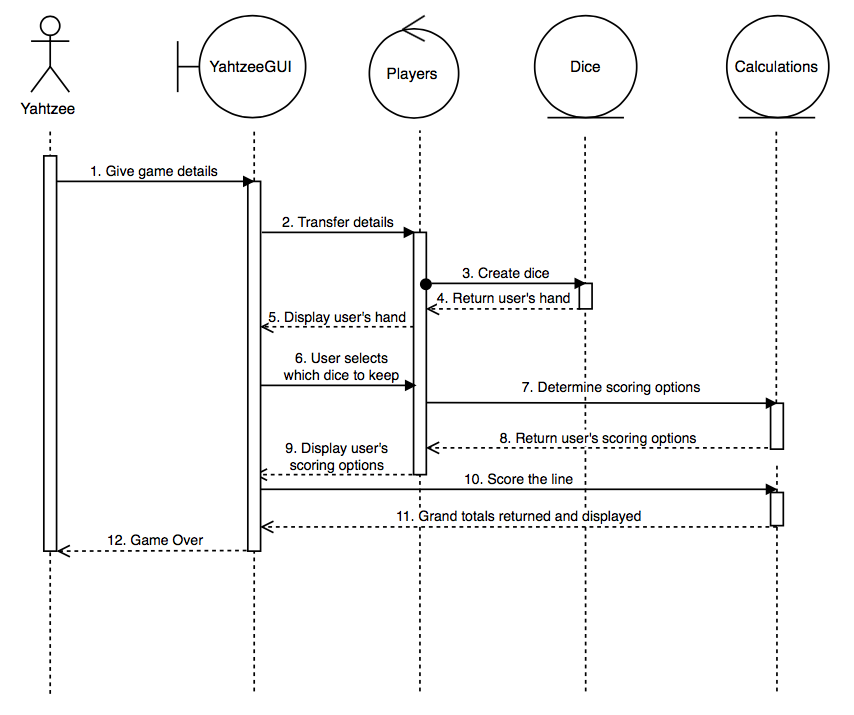
\includegraphics[width=5in]{Graphics/UMLSequenceDiagramScreenshot.png}
\end{center}

\section{Business Function Model (BFM)}     % section 2.3
\underline{Objective:} Play a multiuser game of Gonzaga Men's Basketball Yahtzee in a Graphical User Interface (GUI).

\begin{itemize}

\item Starting a game
	\begin{itemize}
	\item Display the leaderboard (top 3 highest scores in game history)
	\item Display game instructions
	\item Determine number of users
	\item Get the user's name(s)
	\end{itemize}

\item Rolling a hand
	\begin{itemize}
	\item Roll all five dice
	\item Determine if rerolls are available
	\item Prompt the user to keep dice
	\item Reroll all the dice not kept
	\item Determine whether to proceed to scoring (all dice have been kept or all available rolls have been used)
	\end{itemize}

\vspace{.7in}

\item Scoring a hand
	\begin{itemize}
	\item Determine the unused scorelines
	\item Calculate the score for each unused line
	\item Display calculated scores for eligible scoring options
	\item Prompt the user to select a scoring option
	\item Record the score of the selected option to the user's scorecard
	\end{itemize}

\item Finishing a game
	\begin{itemize}
	\item Determine all users have scored all lines
	\item Display the grand total for each user (including the bonus if applicable)
	\item Determine if any user's score qualifies them for the leaderboard
	\item Update the leaderboard if applciable
	\item Thank the user for playing
	\item Inform the user to view the leaderboard or to play again they must close the current window and reload the game
	\end{itemize}
	
\end{itemize}

\section{Functional Requirements}     % section 2.4
\begin{itemize}
\item \textbf{Starting a game:}
At the start of the game, the user has the option to view the leaderboard (top 3 highest scores in game history). The user also has the option to view the game instructions, as well as each basketball player's name, their number, their position, and if they are a starter or bench, as this is key to scoring for the rest of the game. When starting the game, the user will be prompted to select the number of users for the game and then to enter each user's name. As the users play the game, the game will state who's turn it is.
\item \textbf{Rolling a hand:}
	To roll a new hand the first step is to roll all five dice, randomly generating five Gonzaga basketball players. The game will state which roll number the current roll is. The game will prompt the user to select which players to keep in their hand, and which to reroll. The dice that are not kept will be rerolled. At this point, the user's turn will proceed to scoring if one of two conditions is met: either all of the dice have been kept or all available rolls have been used. 
\item \textbf{Scoring a hand:}
	After each turn, the unused scoreboard lines and the value the user is eligible score on those lines is displayed. The user's current score (before scoring the current hand) is displayed. The user is prompted to input a line number they wish to score. The game only allows the user to choose from unused lines. 
\item \textbf{Finishing a game:}
	The game is over once all users have scored all lines. At that point the grand total for each user is displayed (including the bonus, if applicable). If any user's score qualifies them for the leaderboard, the leaderboard will be updated. The users will be thanked for playing and informed to view the leaderboard or to play again they must close the current window and reload the game.
\end{itemize}

\section{User Experience Mockup}     % section 2.5
As part of the planning stages, we created a user experience mockup that showed our design for the look and feel of the user experience. Due to the length of the mockup document, we are only including three samples below from the document (screenshots on the next page). The entire document was turned in separately and previously. In general, we followed our mockup design very closely. It was a great resource for us. The main change we made when actually implementing the program is that we did not use background images. Instead, we used a simple color for the background. This decision was made because we were not seeing the results we anticipated.

\begin{center}
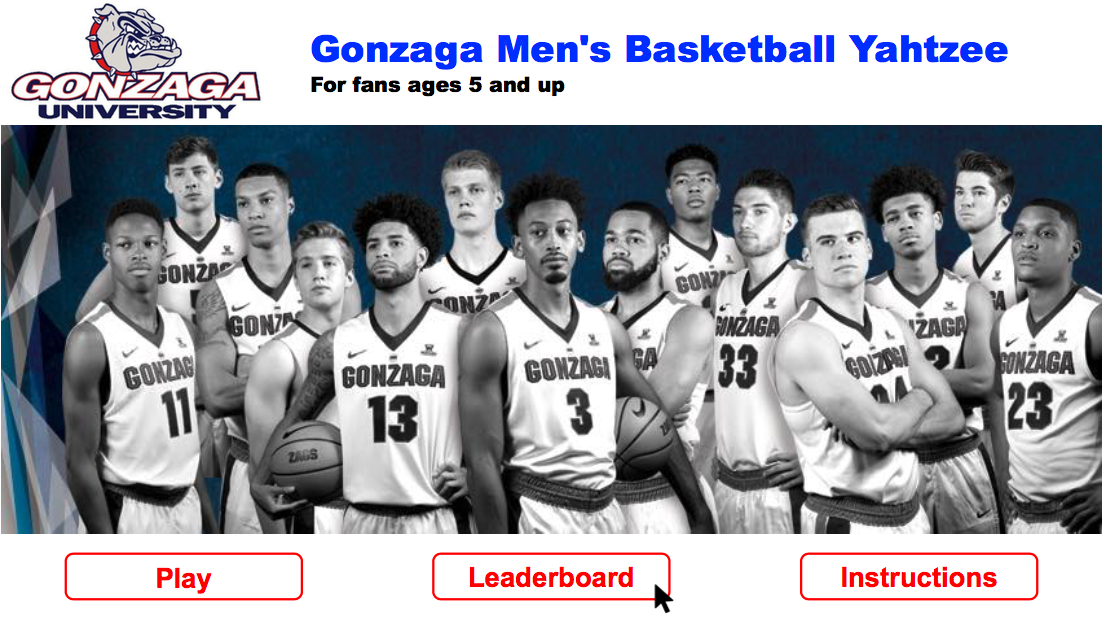
\includegraphics[width=5in]{Graphics/UXMockup-1.png} 
\end{center}

\begin{center}
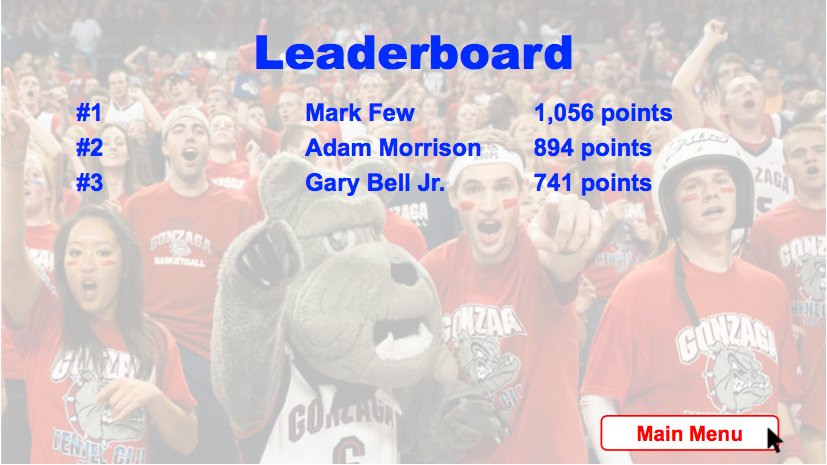
\includegraphics[width=5in]{Graphics/UXMockup-2.png} 
\end{center}

\begin{center}
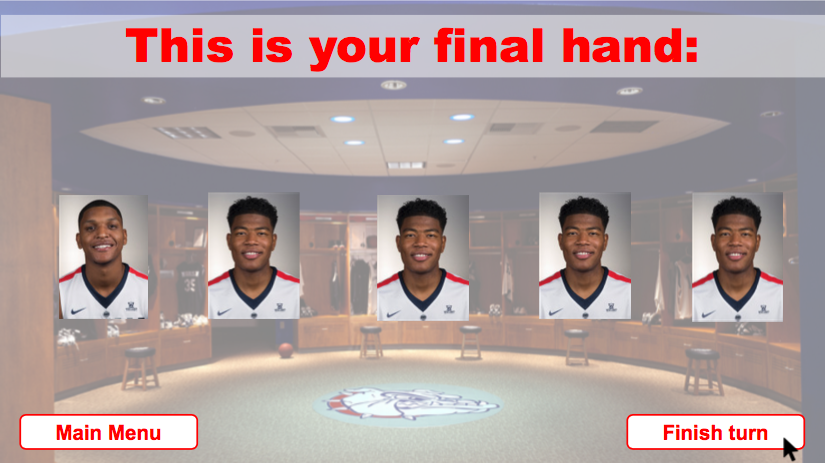
\includegraphics[width=5in]{Graphics/UXMockup-3.png} 
\end{center}


\section{Design Alternative Analysis}     % section 2.6
\begin{itemize}
\item \textbf{Design Alternative Analysis 1}
	\begin{itemize}
	\item \textbf{The issue:} The first problem our group faced with the project is how to incorporate each group member's code from Programming Assignment 6 into a foundation for the group project. Each group member had a successful Programming Assignment 6, so we considered everyone's code. We mainly focused our decision on class design structure and studied each group member's UML diagram. We realized Eugene and Brandon had similar class design structures so for the sake of making a decision we thought of their assignments as one. We evaluated three alternatives.
	\item \textbf{Available alternatives}
		\begin{itemize}
		\item Alternative 1: Keep all of Benjamin's code. There are many methods per class in his design.
		\item Alternative 2: Keep all of Brandon's code. Brandon's code has fewer methods and each method does more work in comparison to Benjamin's code. Eugene's class design structure is similar to Brandon's and will not be evaluated.
		\item Alternative 3: Combine the best aspects of Benjamin's and Brandon's class structure.
		\end{itemize}
	\item \textbf{First alternative}
		\begin{itemize}
		\item In this design, we have four classes: Calculations, Player, Die, and Yahtzee. Each of the classes contains many methods.
		\end{itemize}
	\item \textbf{Pros}
		\begin{itemize}
		\item Since there are many methods in each of the classes the methods do less (in theory, one task). This modularized form of programming generally makes the code easier to read and debug. 
		\item Code can be adapted for multiple users much easier.

		\end{itemize}
	\item \textbf{Cons}
		\begin{itemize}
		\item The design could be considered more complicated because there seems to be more ``going on".
		\item The comments could be improved.
		\begin{center}
		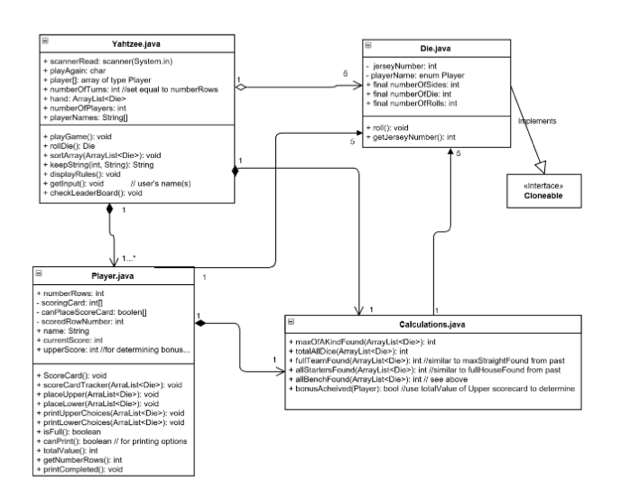
\includegraphics[width=5.5in]{Graphics/DAA1-A1.png} 
		\end{center}
		\end{itemize}
		
	\item \textbf{Second alternative}
		\begin{itemize}
		\item In this class design, we have four classes: Dice, Scorecard, Rules, and Yahtzee.
		\end{itemize}
	\item \textbf{Pros}
		\begin{itemize}
		\item The sorting method is simpler because it does not involve cloneable.
		\item When looking at the UML Class Diagram, this design appears to be simpler than the first alternative.
		\end{itemize}
	\item \textbf{Cons}
		\begin{itemize}
		\item The code is more difficult to read and debug since each method does more than one task.
		\item Many of the methods are static.
		\item There are very few private variables with getter and setter functions.
		\begin{center}
		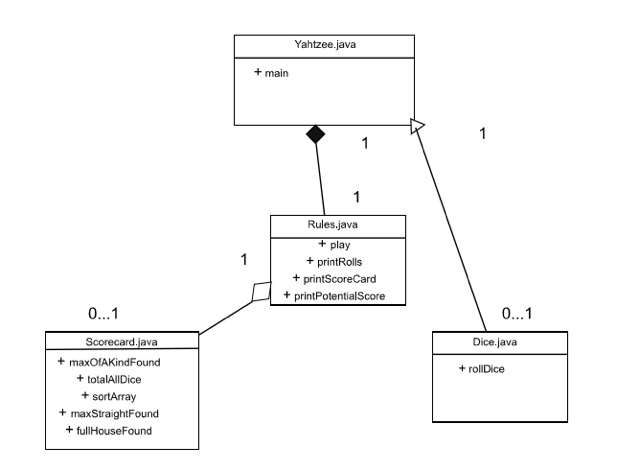
\includegraphics[width=5.4in]{Graphics/DAA1-A2.png} 
		\end{center}
		\end{itemize}
	\item \textbf{Third alternative}
		\begin{itemize}
		\item In this design, we combine Benjamin's and Brandon's Programming Assignment 6 to use as a foundation for the group project.
		\end{itemize}
	\item \textbf{Pros}
		\begin{itemize}
		\item Combines the best aspects of both assignments.
		\end{itemize}
	\item \textbf{Cons}
		\begin{itemize}
		\item No group member is an immediate expert of the code.
		\end{itemize}
	\item \textbf{Decision:} Our group elected to utilize the first alternative. The most significant benefit of the first alternative is that the code adapts with the most ease to a multi-user game. We believe the third alternative would be time-intensive to implement considering variable names, method names, etc. would not match up. Benjamin briefed the entire group on his Programming Assignment 6 code, so that all group members feel comfortable with it and can work with it moving forward.
	\item \textbf{Reflection on choice:} We did make the correct decision by choosing the first alternative. We added one additional class to the original design: YahtzeeGUI. The code from first alternative adapted very well to a multiuser game. Benjamin did a great job of briefing the group on his Programming Assignment 6 code. We all felt very comfortable working with it. \\
	\end{itemize}
	
	\vspace {.5in}
	
\item \textbf{Design Alternative Analysis 2}
	\begin{itemize}
	\item \textbf{The issue:} The problem that our group is encountering is playing the game with more than one user. Our code has a specific player (user) class, which means that we can easily implement more than one user playing the game at a time. When playing a game of Yahtzee in real life, we usually play the game one round at a time, however when we were looking at our code, it works most efficiently when we play the game one user at a time, and then clearing the table, and playing again with the next user.
	\item \textbf{Available alternatives}
		\begin{itemize}
		\item Alternative 1: Users play at the same time
		\item Alternative 2: Users play at different times
		\end{itemize}
	\item \textbf{First alternative}
		\begin{itemize}
		\item In this design, we have the users play at the same time. Figuratively, one user does their turn and then ``hands over" the dice to the next user so that they can do their turn.
		\end{itemize}
		
	
	
	\item \textbf{Pros}
		\begin{itemize}
		\item This option allows the game to finish much quicker, as each user will be allowed to go one at a time. 
		\item Users do not spend as much time waiting, since each user's turns will be a lot closer together rather than one whole game at a time.
		\item The game will feel less like a single user game and will cause users to be more competitive. 
		\end{itemize}
	\item \textbf{Cons}
		\begin{itemize}
		\item This will take much longer to implement.
		\item This will cause more memory to be used and will make our code less efficient.
		\item We want the users to feel more competitive with the leaderboard than with the other users.
		\end{itemize}
	\item \textbf{Second alternative}
		\begin{itemize}
		\item In this design, we have users play one at a time, so that each user plays their own game, and then ``passes" the dice on to the next user.
		\end{itemize}
	\item \textbf{Pros}
		\begin{itemize}
		\item This would be much simpler to implement.
		\item We could get rid of the memory at the end of the round, and then reuse the storage for the next play through of the game.
		\item The users will feel like they are playing against the leaderboard rather than each other.
		\end{itemize}
	\item \textbf{Cons}
		\begin{itemize}
		\item There is a longer wait time between turns since each user must wait until their turn to play the full game.
		\item The is not the traditional way a multiuser (multiplayer) Yahtzee game is played.
		\end{itemize}
		
	\item \textbf{Decision:} We chose to go with alternative one, because although it would be more difficult to implement, we want to have an emphasis on realism. Alternative one will look more similar to a real game of Yahtzee than the other alternative. We also do not want the non-playing users to get bored as they wait for their turn to play the game.
	\item \textbf{Reflection on choice:} We are very happy we decided on the first alternative. Having the users all play the game at the same time and ``passing the dice" back and forth resembles a traditional Yahtzee game. This alternative keeps all of the users engaged with the game. \\
	\end{itemize}

	\vspace {1in}

\item \textbf{Design Alternative Analysis 3}
	\begin{itemize}
	\item \textbf{The issue:} The problem our group is facing is how to implement the GU Men's Basketball Player Numbers. Specifically, we are focusing on how to randomly generate a player and how to sort the players. We initially were planning to use their jersey numbers. However, the problem is that there is a wide range of jersey numbers (anywhere from 1 to 33) and the jersey numbers are not consecutive (i.e. there are players with jersey numbers 1, 2, 3 and 5, but no number 4). This presents a problem because we cannot simply use the random function in Java. We explored two alternatives for this problem.
	\item \textbf{Available alternatives}
		\begin{itemize}
		\item Alternative 1: Utilize a random function with enum values
		\item Alternative 2: Assign consecutive integer values between 1 and 15 to each player and utilize the random function we are familiar with
		\end{itemize}
	\item \textbf{First alternative}
		\begin{itemize}
		\item In this design, we utilize a random function in Java for enum values. Each of the user's names is an enum value, so it would be possible with the function to select one.
		\end{itemize}

\vspace{.2in}

	\item \textbf{Pros}
		\begin{itemize}
		\item This option is rather straightforward and we found examples of how to implement it on the internet. One example we found was randomly selecting a card suit (i.e. Spades, Hearts, Diamonds, Clubs). Our case would be similar.
		\end{itemize}
	\item \textbf{Cons}
		\begin{itemize}
		\item We have never used the random function with enum values, so it is not something we are very familiar with.
		\end{itemize}
		
		An example found on the internet of implementing a random function with enum values is below. We would replace the card suits with the names of the players on the roster and modify the range to be 0 to 14.
	


\belowcaptionskip=-10pt
\begin{lstlisting}
public enum CardSuit
{
	Spades,
	Hearts,
	Diamonds,
	Clubs
}

void Start ()
{
	cardSuit = (CardSuit)Random.Range(0, 3);
}
\end{lstlisting}

		
	\item \textbf{Second alternative}
		\begin{itemize}
		\item In this design, each player on the roster is assigned an integer value between 1 and 15. We utilize the ``normal" and familiar random function to generate a random integer value between 1 and 15. Then, the number generated is matched back to the corresponding player on the roster and further operations are conducted with that player.
		\end{itemize}
	\item \textbf{Pros}
		\begin{itemize}
		\item We completely understand what is happening here. 
		\end{itemize}
	\item \textbf{Cons}
		\begin{itemize}
		\item It will require many lines of code in comparison to the first alternative.
		\end{itemize}
		
		\begin{lstlisting}
/**
* "Rolls" the die by finding a random double between 0.0 and 1.0.
* That result is multiplied by the number of sides + 1 and is
* casted to an integer. A series of conditions are checked, such that
* the result of the roll is matched with its corresponding player
* from the roster. In addition, the player is assigned his 
* corresponding position and status.
* @param N/A
* @returns N/A
* @throws N/A
*/

public void roll(){
	jerseyNumber = (int)(Math.random() * numberOfSides + 1);

       	if(jerseyNumber == 3 || jerseyNumber == 4 || 
	  jerseyNumber == 5 || jerseyNumber == 7 || 
	  jerseyNumber == 13 || jerseyNumber == 15)
		position = "FORWARD";
	else
		position = "GUARD";

	if(jerseyNumber == 9 || jerseyNumber == 10 || 
	  jerseyNumber == 11 || jerseyNumber == 13 || 
	  jerseyNumber == 15)
		status = "STARTER";
	else
		status = "BENCH";

	if(jerseyNumber == 1)
		name = "Joel Ayayi";
	else if(jerseyNumber == 2)
		name = "Jack Beach";
	else if(jerseyNumber == 3)
		name = "Brandon Clarke";
	else if(jerseyNumber == 4)
		name = "Rui Hachimura";
	else if(jerseyNumber == 5)
		name = "Jeremy Jones";
	else if(jerseyNumber == 6)
		name = "Corey Kispert";
	else if(jerseyNumber == 7)
		name = "Jacob Larson";
	else if(jerseyNumber == 8)
		name = "Alex Martin";
	else if(jerseyNumber == 9)
		name = "Silas Melson";
	else if(jerseyNumber == 10)
		name = "Zach Norvell Jr.";
	else if(jerseyNumber == 11)
		name = "Josh Perkins";
	else if(jerseyNumber == 12)
		name = "Brian Pete";
	else if(jerseyNumber == 13)
		name = "Killian Tillie";
	else if(jerseyNumber == 14)
		name = "Jesse Wade";
	else
		name = "Jonathan Williams";
}
\end{lstlisting}
		
		\item \textbf{Decision:} We elected to go with the second alternative because we understood it the best. We know it will work and how it will work, so we were simply just most comfortable with it. The user will not know the difference from what they see and interact with. 
	\item \textbf{Reflection on choice:} We slightly modified what the second alternative means. However, we are happy with the choice we made to choose the second alternative. We do assign an integer value between 1 and 15 to each player and we did utilize the if/else if/else conditions as written above. Instead of matching that value back to the player's corresponding jersey number we instead just use the integer value 1 - 15. We call that assigned value their scaling factor. When we utilized player's jersey numbers in the game, the scoring became ``clunky" because there is a considerable spread between players' jersey numbers (0 - 33). This made certain players way more ``valuable" than we ever intended. We are comfortable with the code behind this alternative. \\
	\end{itemize}

\end{itemize}


\chapter{Testing}           % chapter 3
\section{Test Plan}     % section 3.1

\begin{itemize}

\item \textbf{Starting a game:} At the start of the game, the user has the option to view the leaderboard (top 3 highest scores in game history). The user also has the option to view the game instructions, as well as each basketball player's name, their number, their position, and if they are a starter or bench, as this is key to scoring for the rest of the game. When starting the game, the user will be prompted to select the number of users for the game and then to enter each user's name. As the users play the game, the game will state who's turn it is.
    \begin{center}
    \begin{tabular}{ | l | p{3.5in}  | l | }
    \hline
    \textbf{Requirement ID} & \textbf{Requirement} & \textbf{Verified By} \\ \hline
    1.0 & Starting a game & Test Case 1\\ \hline
    1.1 & Leaderboard displayed (by click) & Test Case 1 Step D\\ \hline
    1.2 & Instructions displayed (by click) & Test Case 1 Step E\\ \hline
    1.3 & Enter number of users & Test Case 1 Step F\\ \hline
    1.4 & Enter user's name(s) & Test Case 1 Step G\\ \hline
    1.5 & Display who's turn it is & Test Case 1 Step H\\ \hline
    \end{tabular}
    \end{center}


\item \textbf{Rolling a game:} To roll a new hand the first step is to roll all five dice, randomly generating five Gonzaga basketball players. The game will state which roll number the current roll is. The game will prompt the user to select which players to keep in their hand, and which to reroll. The dice that are not kept will be rerolled. At this point, the user's turn will proceed to scoring if one of two conditions is met: either all of the dice have been kept or all available rolls have been used. 
    \begin{center}
    \begin{tabular}{ | l | p{3.5in} | l | }
    \hline
    \textbf{Requirement ID} & \textbf{Requirement} & \textbf{Verified By} \\ \hline
    2.0 & Rolling a game& Test Case 2\\ \hline
    2.1 & Roll all the dice by clicking the ball to roll & Test Case 2 Step A\\ \hline
    2.2 & Display the pictures of the five Gonzaga basketball players rolled & Test Case 2 Step B\\ \hline
    2.3 & Display the current roll number & Test Case 2 Step C\\ \hline
    2.4 & User clicks the players they want to keep & Test Case 2 Step D\\ \hline
    2.5 & Appropriate rerolls are made & Test Case 2 Step E\\ \hline
    2.5 & Proceed to scoring if either all the dice have been kept or all rolls have been used, else continue rolling & Test Case 2 Step F\\ \hline
    \end{tabular}
    \end{center}
    
    \vspace{.5in}

\item \textbf{Scoring a hand:} After each turn, the unused scoreboard lines and the value the user is eligible score on those lines is displayed. The user's current score (before scoring the current hand) is displayed. The user is prompted to input a line number they wish to score. The game only allows the user to choose from unused lines. 
    \begin{center}
    \begin{tabular}{ | l | p{3.5in} | l | }
    \hline
    \textbf{Requirement ID} & \textbf{Requirement} & \textbf{Verified By} \\ \hline
    3.0 & Scoring a hand & Test Case 3\\ \hline
    3.1 & Display available lines to score (all lines unused) as well as the points they are eligible to score on each  & Test Case 3 Step A\\ \hline
    3.2 & Display current score (before scoring the current hand) & Test Case 3 Step B\\ \hline
    3.3 & User selects scoreline to score (bad input not accepted) & Test Case 3 Step C\\ \hline
    3.4 & User has/does not have more rolls remaining & Test Case 3 Step D\\ \hline
    3.5 & Case to switch to the next user or case to transition to finishing a game & Test Case 3 Step E\\ \hline
    \end{tabular}
    \end{center}
    
\item \textbf{Finishing a game} The game is over once all users have scored all lines. At that point the grand total for each user is displayed (including the bonus, if applicable). If any user's score qualifies them for the leaderboard, the leaderboard will be updated. The users will be thanked for playing and informed to view the leaderboard or to play again they must close the current window and reload the game.
    \begin{center}
    \begin{tabular}{ | l | p{3.5in} | l | }
    \hline
    \textbf{Requirement ID} & \textbf{Requirement} & \textbf{Verified By} \\ \hline
    4.0 & Finishing a game & Test Case 4\\ \hline
    4.1 & Determine all users have scored all lines & Test Case 4 Step A\\ \hline
    4.2 & Display each user's grand total (including the bonus, if applicable) & Test Case 4 Step B\\ \hline
    4.3 & Determine if any user's score qualifies for the leaderboard & Test Case 4 Step C\\ \hline
    4.4 & Update the leaderboard if necessary & Test Case 4 Step D\\ \hline
    4.5 & Thank the user(s) for playing and inform them to view the leaderboard or to play again they must close the current window and reload the game & Test Case 4 Step E\\ \hline
    \end{tabular}
    \end{center}


\end{itemize}
\textbf{Test Cases}



\renewcommand{\labelenumii}{\Alph{enumii}.}
\renewcommand{\labelenumiii}{\roman{enumiii}.}

	\begin{enumerate}
	\item Test Case 1: New Game
		\begin{enumerate}
		\item Launch game
		\item Display main menu
		\item Provide options for Play, Leaderboard, Instructions
		\item Display the leaderboard when the user clicks ``Leaderboard"
			\begin{enumerate}
			\item Return to the main menu by clicking ``Main Menu"
			\end{enumerate}
		\item Display the instructions when the user clicks ``Instructions"
			\begin{enumerate}
			\item Return to the main menu by clicking ``Main Menu"
			\end{enumerate}
		\item User clicks desired number of users (1-4)
		\item Enter user's name(s)
		\item Display who's turn it is
		\end{enumerate}
		
		\vspace{2.2in}
		
	\item Test Case 2: Rolling a hand
		\begin{enumerate}
		\item Roll all the dice by click the ball to roll
		\item Display the pictures of the five Gonzaga basketball players rolled
		\item Display the current roll number
		\item User clicks the players they want to keep
			\begin{enumerate}
			\item User makes a selection of keeps and rerolls
			\item User decides to keep all of the dice
			\end{enumerate}
		\item Appropriate rerolls are made
		\item Proceed to scoring if either all the dice have been kept or all rolls have been used, else continue rolling
		\end{enumerate}
	\item Test Case 3: Scoring a hand
		\begin{enumerate}
		\item Display available lines to score (all lines unused) as well as the points they are eligible to score on each
		\item Display current score (before scoring the current hand) 
		\item User selects scoreline to score
			\begin{enumerate}
			\item Bad input not accepted
			\end{enumerate}
		\item Determine number of rolls remaining
			\begin{enumerate}
			\item If user has more rolls remaining, return to Test Case Step A
			\item If user does not have rolls remaining, continue...
			\end{enumerate}
		\item Determine how many users still need to play the game
			\begin{enumerate}
			\item If more users still need to play, return to Test Case Step A
			\item If no users still need to play, continue...
			\end{enumerate}
		\end{enumerate}
	\item Test Case 4: Finishing a game
		\begin{enumerate}
		\item Determine all users have scored all lines
		\item Display each user's grand total (including the bonus, if applicable)
		\item Determine if any user's score qualifies for the leaderboard 
		\item Update the leaderboard if necessary
		\item Thank the user(s) for playing and inform them to view the leaderboard or to play again they must close the current window and reload the game
		\end{enumerate}
	
\end{enumerate}

\vspace{2.2in}


\section{JUnit Testing}     % section 3.2
We utilized JUnit, a unit testing framework for the Java programming language, to test our code. The code and screenshots for our JUnit testing have been turned in separately. Below are the screenshots of successful JUnit testing, which includes a small sampling of the code utilized for the test.
\begin{itemize}

\item \textbf{JUnit Testing for Die.java}
\begin{center}
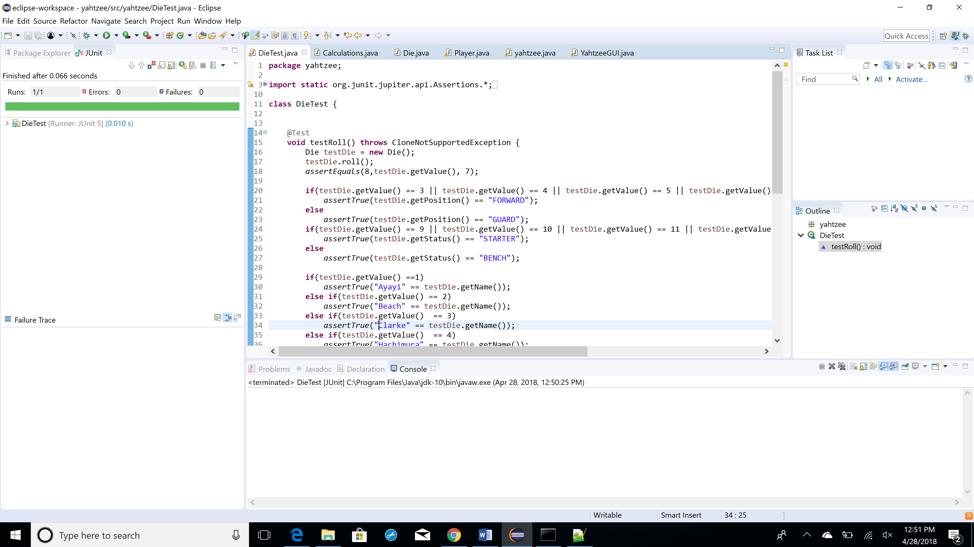
\includegraphics[width=6in]{Graphics/JUnitTestDieTestScreenshot.png}
\end{center}

\vspace{.2in}

\item \textbf{JUnit Testing for Player.java} 
\begin{center}
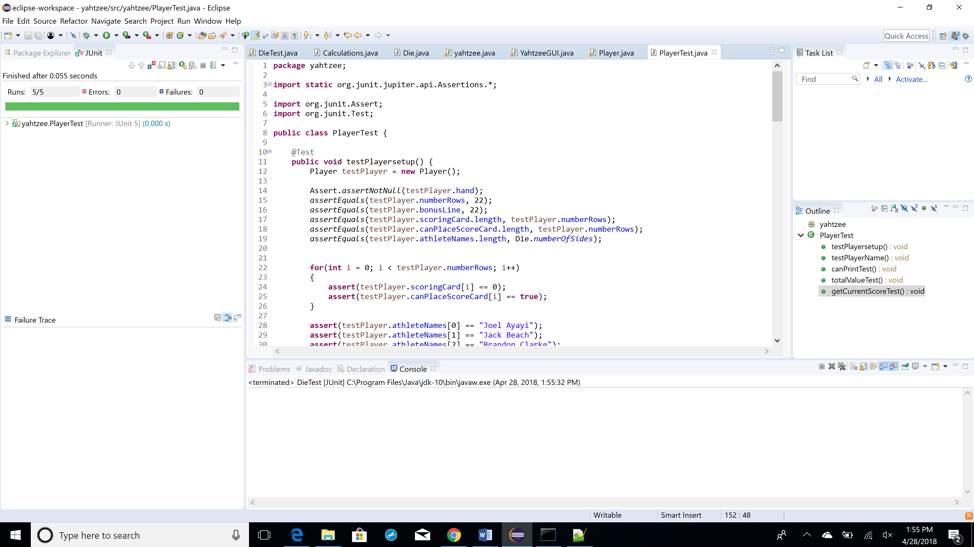
\includegraphics[width=6in]{Graphics/JUnitTestPlayerTestScreenshot.png}
\end{center}

\vspace{.2in}

\item \textbf{JUnit Testing for Calculations.java}
\begin{center}
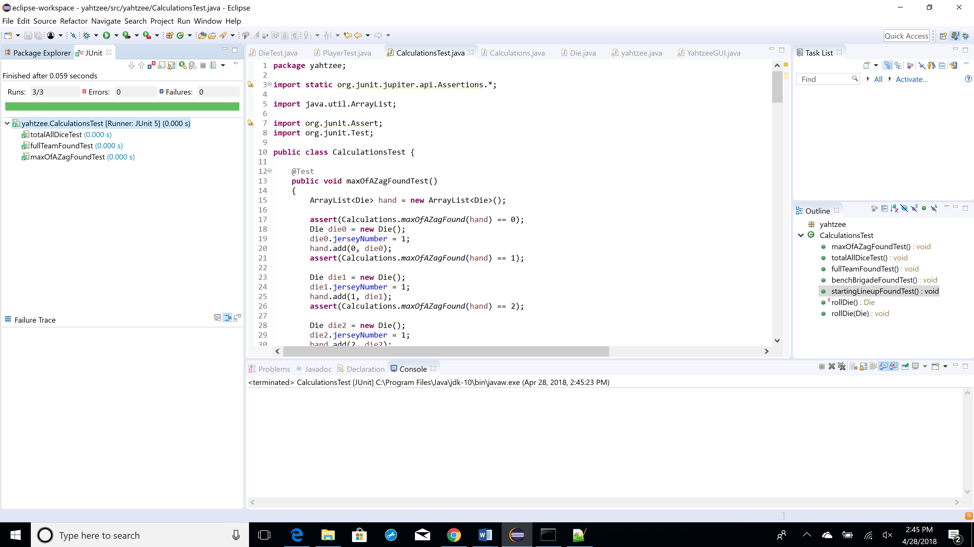
\includegraphics[width=6in]{Graphics/JUnitTestCalculationsTestScreenshot.png}
\end{center}

\end{itemize}




\chapter{Conclusion}           % chapter 4
\section{Reflection on working as a team}     % section 4.1
This was the first long-term project each of us has done. Additionally, this was the first time any of us have worked with a group (we have worked individually or with a partner previously). As a side note, each of us enjoyed this project and liked the long-term approach that justified a serious investment in the project. The three of us enjoyed working together and became closer in the process. We were friends going into the project. Working together did create some frustrations at times (i.e. finding times to meet). However, we did not have any disagreements over how to design or implement the game. All of us were very understanding of each other's opinions and we agreed on a compromise when applicable. In terms of managing the workload, we had a good balance of meeting and working together and dividing work and completing it on our own. Often times there was a pattern we followed for any given task. However, learning how to do the task the first time could be challenging. This is when meeting and working together was beneficial. Then, a group member would feel comfortable finishing the work on their own. Each of us became ``experts" in certain areas of the project and we utilized this to our benefit. We regularly met to review each other's work. We also met at the end of the project to complete a final review.
\section{Existing/remaining issues with the game}     % section 4.2
Fortunately, but not by chance, no issues exist or remain with the game based on our functional requirements. There are improvements that could be made that will be discussed next, however, they are not current issues.
\section{Future work/extensions with the game}     % section 4.3
If we were to continue working on this project beyond the current timeline, there are two main areas we identify for future work/extensions with the game:
\begin{itemize}
\item \textbf{Improved GUI Appearance:} For example, it would look nicer if the panel background was a thematic image, as opposed to a plain color.
\item \textbf{Enhanced User-Input Validation:} For example, it would have been more user-friendly if an error message appeared if the user entered bad input (i.e. a user name that is NOT one word). Our game does not take bad input. The user is allowed to retry and enter valid input. For instance, on the scoring card if the user enters an invalid line to score and clicks submit, the next button does not appear. Once the user does enter valid input, the next button does appear and the user can continue with the game as expected. 
\end{itemize}


\end{document}